% Template for Numbat user manual
% Chris Green, 2018

\documentclass[12pt, a4paper, midday, formal]{csiroreport2017}

\usepackage{graphicx}
\usepackage{amssymb}
\usepackage{amsmath}
\usepackage{booktabs}
\usepackage{tabularx}
\usepackage[small]{caption}
\usepackage[authoryear]{natbib}
\usepackage{authblk}
\usepackage{subcaption}
\usepackage{datetime}

\usepackage{listings} %code extracts
\usepackage{xcolor} %custom colours
\usepackage{mdframed} %nice frames

% pandoc header
\usepackage{lmodern}
\usepackage{amssymb,amsmath}
\usepackage{ifxetex,ifluatex}
\usepackage{fixltx2e} % provides \textsubscript
\ifnum 0\ifxetex 1\fi\ifluatex 1\fi=0 % if pdftex
  \usepackage[T1]{fontenc}
  \usepackage[utf8]{inputenc}
\else % if luatex or xelatex
  \ifxetex
    \usepackage{mathspec}
  \else
    \usepackage{fontspec}
  \fi
  \defaultfontfeatures{Ligatures=TeX,Scale=MatchLowercase}
\fi
% use upquote if available, for straight quotes in verbatim environments
\IfFileExists{upquote.sty}{\usepackage{upquote}}{}
% use microtype if available
\IfFileExists{microtype.sty}{%
\usepackage{microtype}
\UseMicrotypeSet[protrusion]{basicmath} % disable protrusion for tt fonts
}{}
\usepackage{hyperref}
\hypersetup{unicode=true,
            pdfborder={0 0 0},
            breaklinks=true}
\hypersetup{draft}

\urlstyle{tt}

\usepackage{color}
\usepackage{fancyvrb}
\newcommand{\VerbBar}{|}
\newcommand{\VERB}{\Verb[commandchars=\\\{\}]}
\DefineVerbatimEnvironment{Highlighting}{Verbatim}{commandchars=\\\{\}}
% Add ',fontsize=\small' for more characters per line
\newenvironment{Shaded}{}{}
\newcommand{\KeywordTok}[1]{\textcolor[rgb]{0.00,0.44,0.13}{\textbf{{#1}}}}
\newcommand{\DataTypeTok}[1]{\textcolor[rgb]{0.56,0.13,0.00}{{#1}}}
\newcommand{\DecValTok}[1]{\textcolor[rgb]{0.25,0.63,0.44}{{#1}}}
\newcommand{\BaseNTok}[1]{\textcolor[rgb]{0.25,0.63,0.44}{{#1}}}
\newcommand{\FloatTok}[1]{\textcolor[rgb]{0.25,0.63,0.44}{{#1}}}
\newcommand{\ConstantTok}[1]{\textcolor[rgb]{0.53,0.00,0.00}{{#1}}}
\newcommand{\CharTok}[1]{\textcolor[rgb]{0.25,0.44,0.63}{{#1}}}
\newcommand{\SpecialCharTok}[1]{\textcolor[rgb]{0.25,0.44,0.63}{{#1}}}
\newcommand{\StringTok}[1]{\textcolor[rgb]{0.25,0.44,0.63}{{#1}}}
\newcommand{\VerbatimStringTok}[1]{\textcolor[rgb]{0.25,0.44,0.63}{{#1}}}
\newcommand{\SpecialStringTok}[1]{\textcolor[rgb]{0.73,0.40,0.53}{{#1}}}
\newcommand{\ImportTok}[1]{{#1}}
\newcommand{\CommentTok}[1]{\textcolor[rgb]{0.38,0.63,0.69}{\textit{{#1}}}}
\newcommand{\DocumentationTok}[1]{\textcolor[rgb]{0.73,0.13,0.13}{\textit{{#1}}}}
\newcommand{\AnnotationTok}[1]{\textcolor[rgb]{0.38,0.63,0.69}{\textbf{\textit{{#1}}}}}
\newcommand{\CommentVarTok}[1]{\textcolor[rgb]{0.38,0.63,0.69}{\textbf{\textit{{#1}}}}}
\newcommand{\OtherTok}[1]{\textcolor[rgb]{0.00,0.44,0.13}{{#1}}}
\newcommand{\FunctionTok}[1]{\textcolor[rgb]{0.02,0.16,0.49}{{#1}}}
\newcommand{\VariableTok}[1]{\textcolor[rgb]{0.10,0.09,0.49}{{#1}}}
\newcommand{\ControlFlowTok}[1]{\textcolor[rgb]{0.00,0.44,0.13}{\textbf{{#1}}}}
\newcommand{\OperatorTok}[1]{\textcolor[rgb]{0.40,0.40,0.40}{{#1}}}
\newcommand{\BuiltInTok}[1]{{#1}}
\newcommand{\ExtensionTok}[1]{{#1}}
\newcommand{\PreprocessorTok}[1]{\textcolor[rgb]{0.74,0.48,0.00}{{#1}}}
\newcommand{\AttributeTok}[1]{\textcolor[rgb]{0.49,0.56,0.16}{{#1}}}
\newcommand{\RegionMarkerTok}[1]{{#1}}
\newcommand{\InformationTok}[1]{\textcolor[rgb]{0.38,0.63,0.69}{\textbf{\textit{{#1}}}}}
\newcommand{\WarningTok}[1]{\textcolor[rgb]{0.38,0.63,0.69}{\textbf{\textit{{#1}}}}}
\newcommand{\AlertTok}[1]{\textcolor[rgb]{1.00,0.00,0.00}{\textbf{{#1}}}}
\newcommand{\ErrorTok}[1]{\textcolor[rgb]{1.00,0.00,0.00}{\textbf{{#1}}}}
\newcommand{\NormalTok}[1]{{#1}}
\IfFileExists{parskip.sty}{%
\usepackage{parskip}
}{% else
\setlength{\parindent}{0pt}
\setlength{\parskip}{6pt plus 2pt minus 1pt}
}
\setlength{\emergencystretch}{3em}  % prevent overfull lines
\providecommand{\tightlist}{%
  \setlength{\itemsep}{0pt}\setlength{\parskip}{0pt}}
% Redefines (sub)paragraphs to behave more like sections
\ifx\paragraph\undefined\else
\let\oldparagraph\paragraph
\renewcommand{\paragraph}[1]{\oldparagraph{#1}\mbox{}}
\fi
\ifx\subparagraph\undefined\else
\let\oldsubparagraph\subparagraph
\renewcommand{\subparagraph}[1]{\oldsubparagraph{#1}\mbox{}}
\fi

\definecolor{light-gray}{gray}{0.95} %the shade of grey that stack exchange uses
\surroundwithmdframed[nobreak=true,backgroundcolor=light-gray,linecolor=light-gray,skipabove=11,skipbelow=11]{lstlisting}
\surroundwithmdframed[nobreak=true,backgroundcolor=light-gray,linecolor=light-gray,skipabove=11,skipbelow=11]{Shaded}

\lstset{basicstyle=\ttfamily\footnotesize,breaklines=true}
\lstset{backgroundcolor=\color{light-gray}}

\setcounter{tocdepth}{2}

\setlength{\belowcaptionskip}{\abovecaptionskip}

% Alert environment
\newenvironment{alert}{%
\par
\noindent
\textbf{Note:}
\noindent}
{}

\surroundwithmdframed[backgroundcolor=light-colour,linecolor=light-colour,skipabove=11,skipbelow=11]{alert}
\surroundwithmdframed[backgroundcolor=light-gray,linecolor=light-gray,skipabove=11,skipbelow=11]{verbatim}

\docdivision[ENERGY]
\doctitle[{\huge Numbat}]
\docsubtitle[High-resolution simulations of density-driven convective mixing in porous media]
\docauthors[\vspace{1cm} Christopher Green]
\docreportnum[Report Number EP186698]
\docreportdate[\monthname, \the\year]
\doccopyrightyear[2018]

\docfootertitle[]

\docbusinessunit[CSIRO Energy \\
71 Normanby Road, Clayton VIC, 3168, Australia \\
Private Bag 10, Clayton South VIC, 3169, Australia \\
Telephone: +61 3 9545 2777 \\
Fax: +61 3 9545 8380]

\docfurtherinfoA[CSIRO Energy]{Chris Green}
{+61 3 9545 8371}{chris.green@csiro.au}{}{www.csiro.au}

\begin{document}
\pagenumbering{roman}
\clearpage
\listoffigures
% \clearpage
% \listoftables
\clearpage
\pagenumbering{arabic}

%%%%%%%%%%%%%%%%%%%%%%%%%%%%%%%%%%%%%%%%%%%%%%%%%%%%
%
% Introduction
%
%%%%%%%%%%%%%%%%%%%%%%%%%%%%%%%%%%%%%%%%%%%%%%%%%%%%
\section{Numbat}

Numbat is an open-source MOOSE\footnote{www.mooseframework.org} application for high-resolution simulations of buoyancy-driven convection in porous media in both two and three dimensions.

\begin{figure}[ht]
\begin{center}
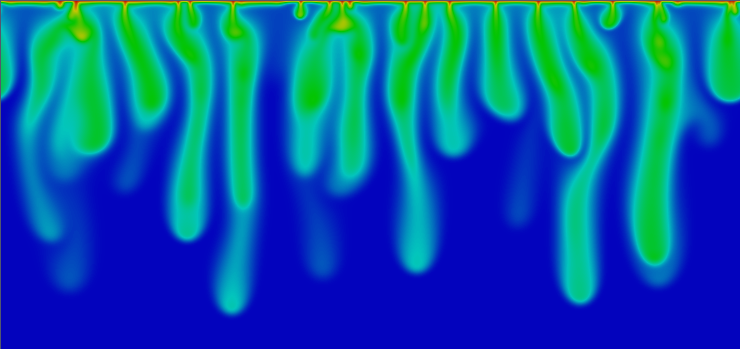
\includegraphics[width=\textwidth]{../content/media/convection.png}
\caption{Density-driven convective mixing in porous media}
\label{fig:convection}
\end{center}
\end{figure}

As a MOOSE app, it provides access to powerful MOOSE features such as adaptive mesh refinement, hybrid parallelism, both continuous and discontinuous Galerkin methods, and much more, all wrapped in a simple interface.

Numat solves the coupled convection-diffusion and Darcy equations with the Boussinesq approximation using the finite element method.

Several formulations are available: from the full, dimensional governing equations, to a dimensionless streamfunction formulation.

\subsection{Development and testing}

Numbat is developed on GitHub\footnote{www.github.com/cpgr/numbat} by CSIRO\footnote{www.csiro.au}. It follows the MOOSE continuous
integration/continuous development philosphy, where changes are merged into the master branch of the repository only after being tested
succesfully against the automatic test suite provided by Numbat.

Numbat is also part of the upstream MOOSE testing procedure, where all changes to MOOSE are tested against
Nubmat (as well as other MOOSE applications) to ensure no conflicts.

\subsection{User manual version}

Due to this development philosphy, Numbat does not feature the concept of software versions. A consequence of this
is that there are no version label applied to this user manual. This documentation is updated as new features and
examples are added to the Numbat application.

The most up-to-date version of this document is always available on the Numbat website.

%%%%%%%%%%%%%%%%%%%%%%%%%%%%%%%%%%%%%%%%%%%%%%%%%%%%
%
% Included files
%
%%%%%%%%%%%%%%%%%%%%%%%%%%%%%%%%%%%%%%%%%%%%%%%%%%%%
\include{introduction}
\include{governing_equations}
\include{getting_started}
\include{implementation}
\include{input_file_syntax}
\include{running_numbat}
\include{example2D}
\include{example3D}
\include{contributing}

%%%%%%%%%%%%%%%%%%%%%%%%%%%%%%%%%%%%%%%%%%%%%%%%%%%%
%
% BIBLIOGRAPHY
%
%%%%%%%%%%%%%%%%%%%%%%%%%%%%%%%%%%%%%%%%%%%%%%%%%%%%
\clearpage
\bibliography{../content/bib/numbat.bib}
\bibliographystyle{authordate1}

\end{document}
